\section{Evaluation}\label{sec:eval}
% 英文版原始算法内容(如无legend相关内容则无需更改)

In this section, we assess Fidelius's performance through comprehensive experiments. Initially, we gauge its time consumption by executing CPU-intensive and I/O-intensive tasks separately. Subsequently, we conduct a performance comparison between Fidelius and alternative solutions that execute analysis programs in the Ethereum Virtual Machine (EVM). Our experiments are conducted on a machine equipped with an Intel(R) Core(TM) i5-10400F CPU boasting 12 cores at 2.9 GHz, 16 GBytes of RAM, and a 12 MByte cache. Unless otherwise stated, each experiment is repeated 1,000 times to calculate the average value.

\subsection{CPU-Intensive Task}
To evaluate Fidelius's performance on CPU-intensive tasks, we implement a neural network algorithm with three layers and 128 hidden units, designed to recognize handwritten digits using the MNIST dataset~\cite{mnist}. We report both the time consumption and accuracy of the algorithm. Additionally, we deploy the algorithm on raw CPU (without SGX) for comparison. The key differences between the Fidelius-based algorithm and the raw CPU-based algorithm include:
\begin{itemize}
  \item Random library. The Fidelius-based algorithm utilizes a random library based on Intel SGX, whereas the raw CPU-based algorithm relies on the C++ random library.
  \item Data decryption. Fidelius requires decryption of sealed data before initiating the algorithm, incurring additional processing time. Conversely, the raw CPU-based algorithm can directly access plaintext data.
\end{itemize}
Both for Fidelius and raw CPU, we maintain a fixed number of test sets at 1,000 while incrementally increasing the number of training sets from 10,000 to 50,000. For each training set, we execute the algorithm with epochs set to 100 and 200, respectively.


\begin{figure*}[h]
\centering
{
  \setlength{\tabcolsep}{0pt}
  \begin{tabular}{cccc}
\subfloat[epoch = 100]{
  \scalebox{0.39}{
  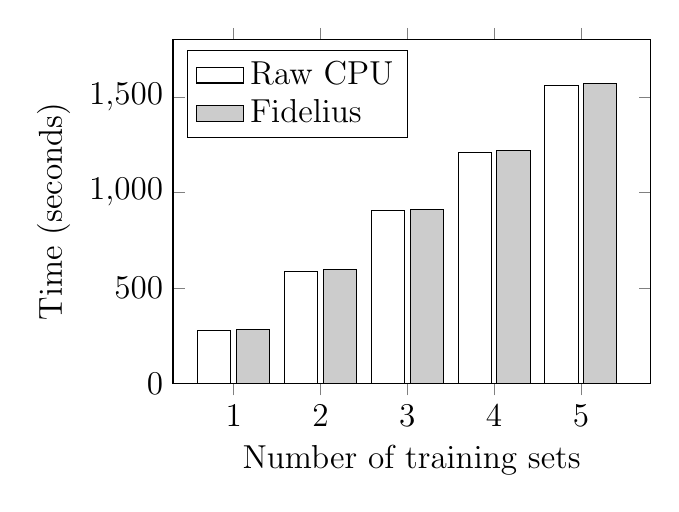
\begin{tikzpicture}
    
\begin{axis}[
  compat=newest,
  legend style={
     legend columns=1,
     font=\large,
     legend pos=north west},
  ybar,
  bar width=12pt,
  ymin=0,
  ymax=1800,
  xmin=0.3,
  xmax=5.8,
  scale only axis,
  xticklabels={\bench{\large 1}, \bench{\large 2}, \bench{\large 3},
    \bench{\large 4}, \bench{\large 5}
  },
  ylabel={Time (seconds)
  },
    xlabel=Number of training sets,
    xtick=data,
    width=0.5\textwidth,
    height=0.36\textwidth,
    every axis/.append style={font=\large,
      label style={font=\large},
      tick label style={font=\large}
    }
  ]
\addplot [area legend] coordinates{
  (1, 278.258)
  (2, 587.359)
  (3, 905.65)
  (4, 1208.9)
  (5, 1562.5)
};
\addplot [fill=black!20,area legend] coordinates{
  (1, 282)
  (2, 595.27)
  (3, 909.03)
  (4, 1219.71)
  (5, 1570)
};
\legend{[right]{Raw CPU}, [right]{Fidelius}}
\end{axis}
\end{tikzpicture}}
} &
\subfloat[epoch = 200]{
  \scalebox{0.39}{
  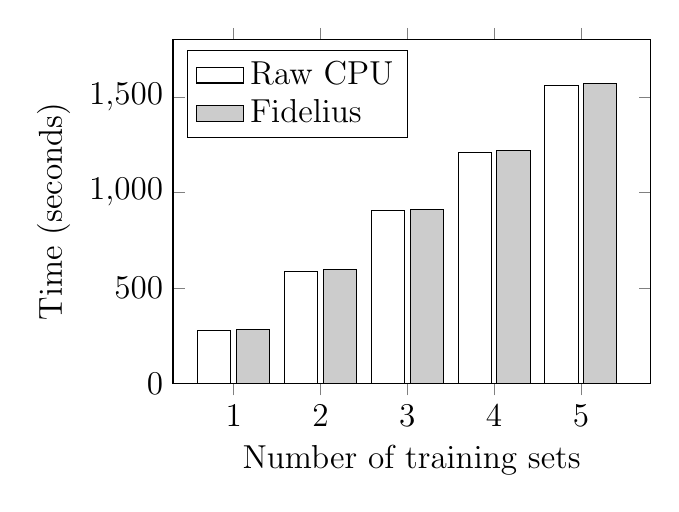
\begin{tikzpicture}
    
\begin{axis}[
  compat=newest,
  legend style={
     legend columns=1,
     font=\large,
     legend pos=north west},
  ybar,
  bar width=12pt,
  ymin=0,
  ymax=1800,
  xmin=0.3,
  xmax=5.8,
  scale only axis,
  xticklabels={\bench{\large 1}, \bench{\large 2}, \bench{\large 3},
    \bench{\large 4}, \bench{\large 5}
  },
  ylabel={Time (seconds)
  },
    xlabel=Number of training sets,
    xtick=data,
    width=0.5\textwidth,
    height=0.36\textwidth,
    every axis/.append style={font=\large,
      label style={font=\large},
      tick label style={font=\large}
    }
  ]
\addplot [area legend] coordinates{
  (1, 278.258)
  (2, 587.359)
  (3, 905.65)
  (4, 1208.9)
  (5, 1562.5)
};
\addplot [fill=black!20,area legend] coordinates{
  (1, 282)
  (2, 595.27)
  (3, 909.03)
  (4, 1219.71)
  (5, 1570)
};
\legend{[right]{Raw CPU}, [right]{Fidelius}}
\end{axis}		
\end{tikzpicture}}
} &
\subfloat[epoch = 100]{
  \scalebox{0.39}{
  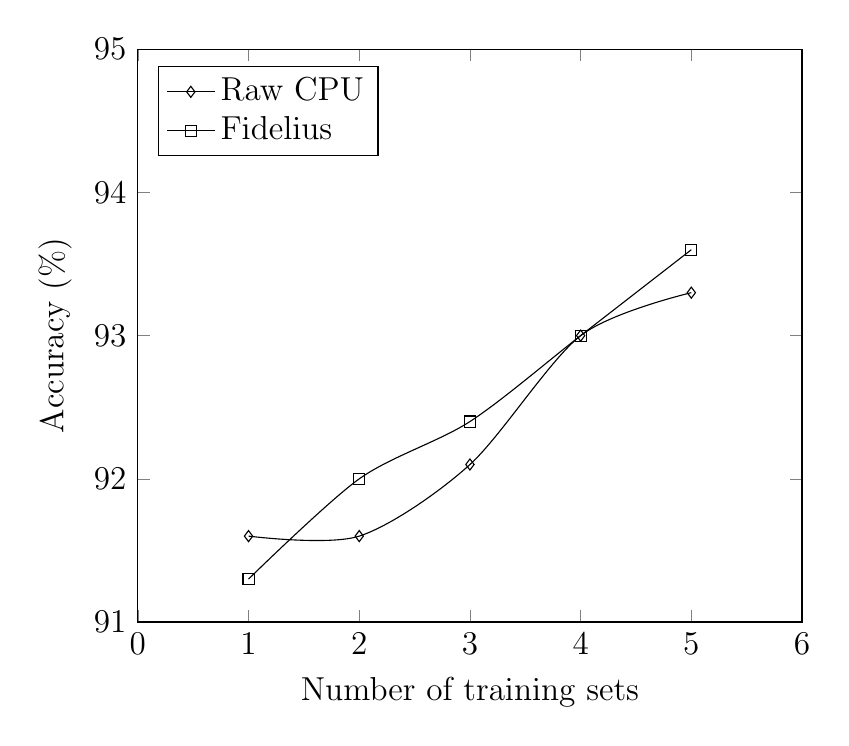
\begin{tikzpicture}
    
\large
\pgfplotsset{
    scale only axis,
    xmin=0, xmax=6,
    compat=newest,
    legend pos=north west,
}

\begin{axis}[
  %axis y line*=left,
  %scaled y ticks=base 10:2,
  %ymin=0, ymax=0.0004,
  %ymin=0, ymax=0.008,
  ymin=91, ymax=95,
  xlabel=Number of training sets,
  %width=0.4\textwidth,
  %height=0.6\textwidth,
  ylabel=Accuracy (\%),
]

\addplot[smooth,mark=diamond]
  coordinates{
    (1,91.6)
    (2,91.6)
    (3,92.1)
    (4,93.0)
    (5,93.3)
}; \label{plot_raw}

\addplot[smooth,mark=square]
  coordinates{
    (1,91.3)
    (2,92.0)
    (3,92.4)
    (4,93.0)
    (5,93.6)
  }; \label{plot_fid}



  \addlegendimage{/pgfplots/refstyle=plot_raw}\addlegendentry[right]{Raw CPU}
  \addlegendimage{/pgfplots/refstyle=plot_fid}\addlegendentry[right]{Fidelius}

\end{axis}
\end{tikzpicture}}
} &
\subfloat[epoch = 200]{
  \scalebox{0.39}{
  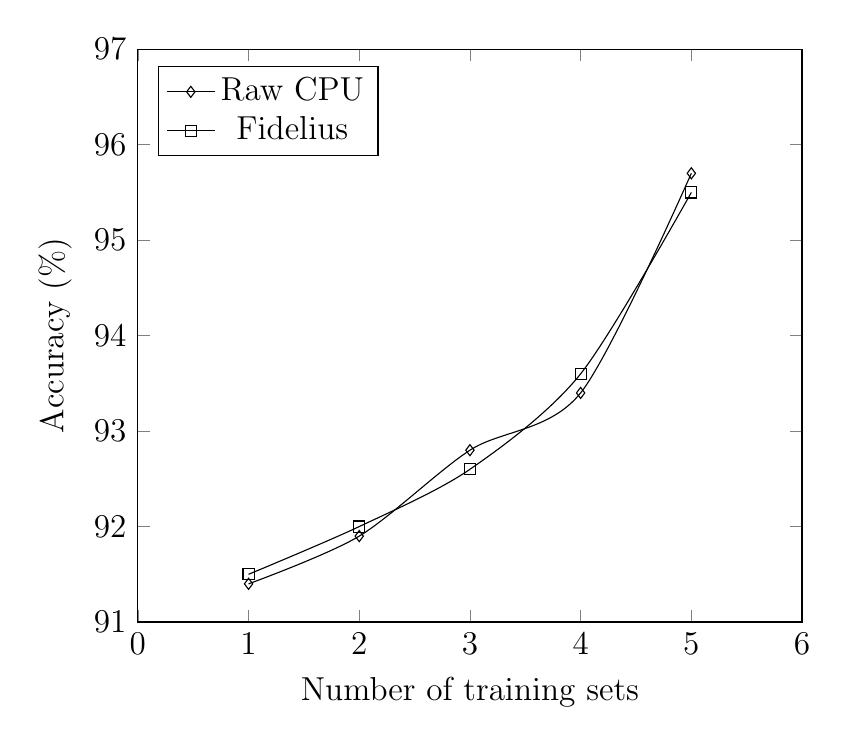
\begin{tikzpicture}
    
\large
\pgfplotsset{
    scale only axis,
    xmin=0, xmax=6,
    compat=newest,
    legend pos=north west,
}

\begin{axis}[
  %axis y line*=left,
  %scaled y ticks=base 10:2,
  %ymin=0, ymax=0.0004,
  %ymin=0, ymax=0.008,
  ymin=91, ymax=97,
  xlabel=Number of training sets,
  %width=0.4\textwidth,
  %height=0.6\textwidth,
  ylabel=Accuracy (\%),
]

\addplot[smooth,mark=diamond]
  coordinates{
    (1,91.4)
    (2,91.9)
    (3,92.8)
    (4,93.4)
    (5,95.7)
}; \addlegendentry{Raw CPU}

\addplot[smooth,mark=square]
  coordinates{
    (1,91.5)
    (2,92.0)
    (3,92.6)
    (4,93.6)
    (5,95.5)
  }; \addlegendentry{Fidelius}

\end{axis}
\end{tikzpicture}}
} \\
\end{tabular}
}
  \caption{\small Time Consumption and Accuracy of CPU-Intensive Task.}
\label{fig:cpu_intensive}
\end{figure*}


Figures~\ref{fig:cpu_intensive}(a) and~\ref{fig:cpu_intensive}(b) illustrate the time consumption of the algorithms running on Fidelius and raw CPU with varying epochs. As the number of training sets increases, the time consumption of the algorithms on both Fidelius and raw CPU shows a linear growth trend. However, the time consumption difference between these two algorithms is minimal. Specifically, it is observed that the execution time on Fidelius is only 2\% longer than that of raw CPU, primarily due to data decryption overhead.

Figures~\ref{fig:cpu_intensive}(c) and~\ref{fig:cpu_intensive}(d) show the accuracy of algorithms on Fidelius and raw CPU over different epochs, with both achieving over 91\% accuracy. At 100 epochs, accuracy fluctuates slightly, but with no marked difference between the platforms. At 200 epochs, both algorithms converge with nearly identical accuracies. Fidelius shows a marginal 2\% increase in time consumption compared to raw CPU but maintains similar accuracy levels, demonstrating comparable performance in CPU-intensive tasks.


\subsection{I/O-Intensive Task}\label{subsec:io_intensive}
To evaluate the time efficiency of Fidelius in handling I/O-intensive tasks, we tested an algorithm that searches for a target string within a file over 1 GByte on both Fidelius and raw CPU platforms. Time consumption depends on data loading and string searching, with additional time required on Fidelius due to data decryption. Given Intel SGX's constraints in Fidelius, we set data loading block sizes to 64 KBytes and 256 KBytes and varied the number of data lines from 1 to 128 and 1 to 256 for each block size to measure time efficiency.



\begin{figure}[h]
  \centering
{
\begin{tabular}{cc}
      \subfloat[Data block size = 64 KBytes]{
        \scalebox{0.39}{
          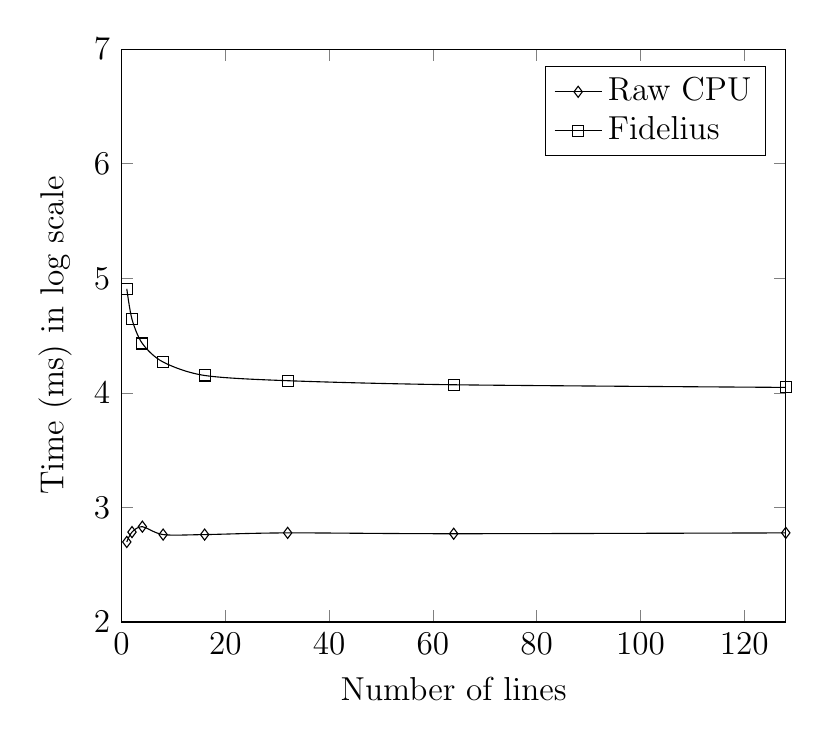
\begin{tikzpicture}
            
\large
\pgfplotsset{
    scale only axis,
    xmin=0, xmax=128,
    compat=newest,
    legend pos=north east,
}

\begin{axis}[
  %axis y line*=left,
  %scaled y ticks=base 10:2,
  %ymin=0, ymax=0.0004,
  %ymin=0, ymax=0.008,
  ymin=2, ymax=7,
  xlabel=Number of lines,
  %width=0.4\textwidth,
  %height=0.6\textwidth,
  ylabel=Time (ms) in log scale,
]

\addplot[smooth,mark=diamond]
  coordinates{
    (1,2.6990) %log10(500)
    (2,2.7853) %log10(610)
    (4,2.8325) %log10(680)
    (8,2.7634) %log10(580)
    (16,2.7634) %log10(580)
    (32,2.7782) %log10(600)
    (64,2.7709) %log10(590)
    (128,2.7782) %log10(600)
}; \label{plot_raw}

\addplot[smooth,mark=square]
  coordinates{
    (1,4.9085) %log10(81000)
    (2,4.6435) %log10(44000)
    (4,4.4314) %log10(27000)
    (8,4.2695) %log10(18600)
    (16,4.1523) %log10(14200)
    (32,4.1065) %log10(12780)
    (64,4.0711) %log10(11780)
    (128,4.0481) %log10(11170)
  }; \label{plot_fid}



  \addlegendimage{/pgfplots/refstyle=plot_raw}\addlegendentry[right]{Raw CPU}
  \addlegendimage{/pgfplots/refstyle=plot_fid}\addlegendentry[right]{Fidelius}

\end{axis}
          \end{tikzpicture}
        }
      } &
      \subfloat[Data block size = 256 KBytes]{
        \scalebox{0.39}{
          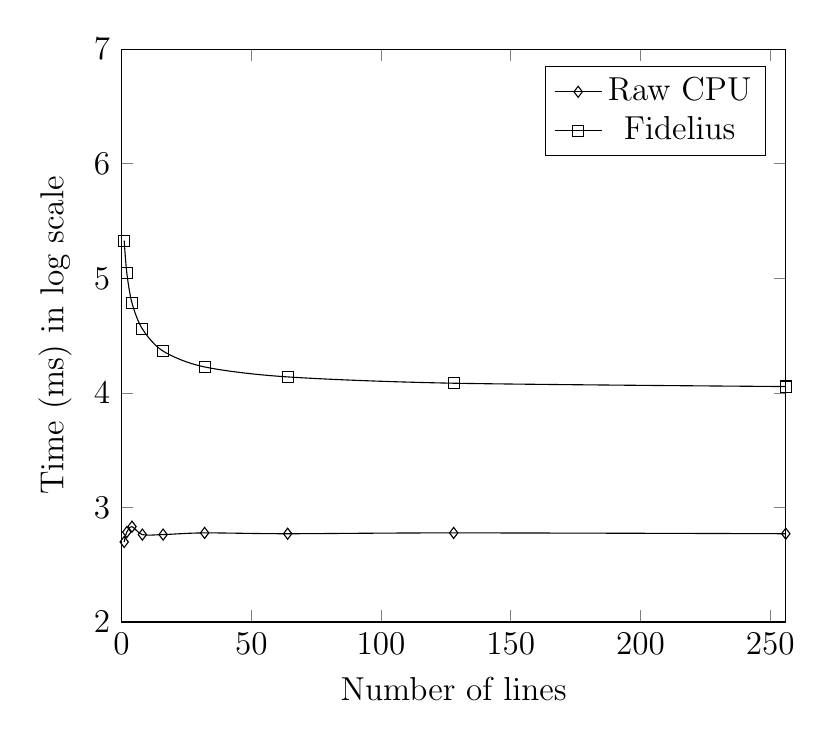
\begin{tikzpicture}
            
\large
\pgfplotsset{
    scale only axis,
    xmin=0, xmax=256,
    compat=newest,
    legend pos=north east,
}

\begin{axis}[
  %axis y line*=left,
  %scaled y ticks=base 10:2,
  %ymin=0, ymax=0.0004,
  %ymin=0, ymax=0.008,
  ymin=2, ymax=7,
  xlabel=Number of lines,
  %width=0.4\textwidth,
  %height=0.6\textwidth,
  ylabel=Time (ms) in log scale,
]
1	0.5	    213
2	0.61	111.78
4	0.68	61.04
8	0.58	36.2
16	0.58	23.16
32	0.6	    16.85
64	0.59	13.79
128	0.6	    12.15
256	0.59	11.36
\addplot[smooth,mark=diamond]
  coordinates{
    (1,2.6990) %log10(500)
    (2,2.7853) %log10(610)
    (4,2.8325) %log10(680)
    (8,2.7634) %log10(580)
    (16,2.7634) %log10(580)
    (32,2.7782) %log10(600)
    (64,2.7709) %log10(590)
    (128,2.7782) %log10(600)
    (256, 2.7709) %log10(590)
}; \addlegendentry{Raw CPU}

\addplot[smooth,mark=square]
  coordinates{
    (1,5.3284) %log10(213000)
    (2,5.0484) %log10(111780)
    (4,4.7856) %log10(61040)
    (8,4.5587) %log10(36200)
    (16,4.3647) %log10(23160)
    (32,4.2266) %log10(16850)
    (64,4.1396) %log10(13790)
    (128,4.0846) %log10(12150)
    (256,4.0554) %log10(11360)
  }; \addlegendentry{Fidelius}

\end{axis}
          \end{tikzpicture}
        }
      }    \\
\end{tabular}
  }
  \caption{\small Time Consumption of I/O-Intensive Task.}
  \label{fig:io_intensive}
\end{figure}

Figure~\ref{fig:io_intensive} shows the time efficiency of Fidelius compared to raw CPU across different data block sizes. Fidelius shows a significant reduction in time consumption as the number of lines read increases. For instance, with a block size of 64 KBytes, the time taken by Fidelius drops from 81 seconds (for 1 line) to 11 seconds (for 128 lines). Similarly, with a block size of 256 KBytes, it reduces from 213 seconds (for 1 line) to 10 seconds (for 256 lines). Increasing the block size to 256 KBytes further optimizes Fidelius's performance. Despite improvements, a gap remains in time consumption between Fidelius and raw CPU, largely due to the decryption process in I/O-intensive tasks.

\subsection{Performance Comparison}\label{subsec:evm_cmp}
In this section, we compare the performance of Fidelius with SDTE~\cite{dai2019sdte}, which uses a \textit{k}-nearest neighbors (\textit{k}-NN) algorithm as an Ethereum smart contract to execute machine learning tasks on the Ethereum Virtual Machine (EVM). We implement the \textit{k}-NN algorithm on both Fidelius and raw CPU to evaluate each solution's time consumption, using the Titanic~\cite{titanic} dataset from Kaggle as input.

To evaluate the \textit{k}-NN algorithm's execution time on the Ethereum Virtual Machine (EVM), we deployed the \textit{k}-NN smart contract on Ganache, a personal Ethereum blockchain. The reported time consumption for \textit{k}-NN on the EVM focuses solely on the execution time, excluding any time spent on transaction broadcasting or committing. We also exclude the time required to upload the Titanic dataset to the blockchain, as the \textit{k}-NN contract uses on-chain data. Due to EVM's memory limits, the \textit{k}-NN algorithm cannot handle more than 60 test sets, hence we limit test sets to 10-60 while keeping training sets at 100.


\begin{figure}[h]
\centering
\scalebox{.8}
{
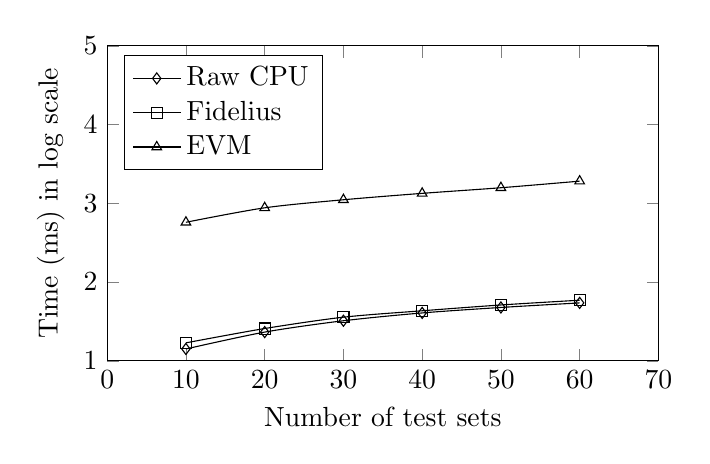
\begin{tikzpicture}
    
\pgfplotsset{
    scale only axis,
    xmin=0, xmax=70,
    ymin=1, ymax=5,
    compat=newest,
    legend pos=north west,
}

\begin{axis}[
  %axis y line*=left,
  %scaled y ticks=base 10:2,
  x=0.1cm,
  y=1cm,
  xlabel=Number of test sets,
  %width=0.4\textwidth,
  %height=0.6\textwidth,
  ylabel=Time (ms) in log scale,
]

\addplot[smooth,mark=diamond]
  coordinates{
    (10,1.1501) %log10(14.13)
    (20,1.3642) %log10(23.13)
    (30,1.5083) %log10(32.23)
    (40,1.6076) %log10(40.51)
    (50,1.6771) %log10(47.54)
    (60,1.7350) %log10(54.32)
}; \label{plot_raw}

\addplot[smooth,mark=square]
  coordinates{
    (10,1.2276) %log10(16.89)
    (20,1.4096) %log10(25.68)
    (30,1.5535) %log10(35.77)
    (40,1.6350) %log10(43.15)
    (50,1.7088) %log10(51.14)
    (60,1.7693) %log10(58.79)
  }; \label{plot_fid}

\addplot[smooth,mark=triangle]
  coordinates{
    (10,2.7589) %log10(574)
    (20,2.9425) %log10(876)
    (30,3.0449) %log10(1109)
    (40,3.1261) %log10(1337)
    (50,3.1976) %log10(1576)
    (60,3.2813) %log10(1911)
  }; \label{plot_evm}


  \addlegendimage{/pgfplots/refstyle=plot_raw}\addlegendentry[right]{Raw CPU}
  \addlegendimage{/pgfplots/refstyle=plot_fid}\addlegendentry[right]{Fidelius}
  \addlegendimage{/pgfplots/refstyle=plot_evm}\addlegendentry[right]{EVM}

\end{axis}
\end{tikzpicture}
}
  

  \caption{\small Time Consumption on Raw CPU, Fidelius and EVM.}
\label{fig:knn_cmp}
\end{figure}

Figure~\ref{fig:knn_cmp} shows the time consumption of the \textit{k}-NN algorithm on raw CPU, Fidelius, and the Ethereum Virtual Machine (EVM), with the latter taking roughly 30 times longer than the others. Additionally, EVM executions often fail when testing more than 60 sets due to memory constraints, highlighting the difficulties of running complex machine learning algorithms with large datasets on the EVM, as also noted in previous studies about Ethereum's memory limits~\cite{dinh2017blockbench}. In contrast, Fidelius provides a more reliable and stable environment for sophisticated machine learning tasks.
